\documentclass[tikz]{standalone}
\usetikzlibrary{automata,positioning}
\begin{document}
  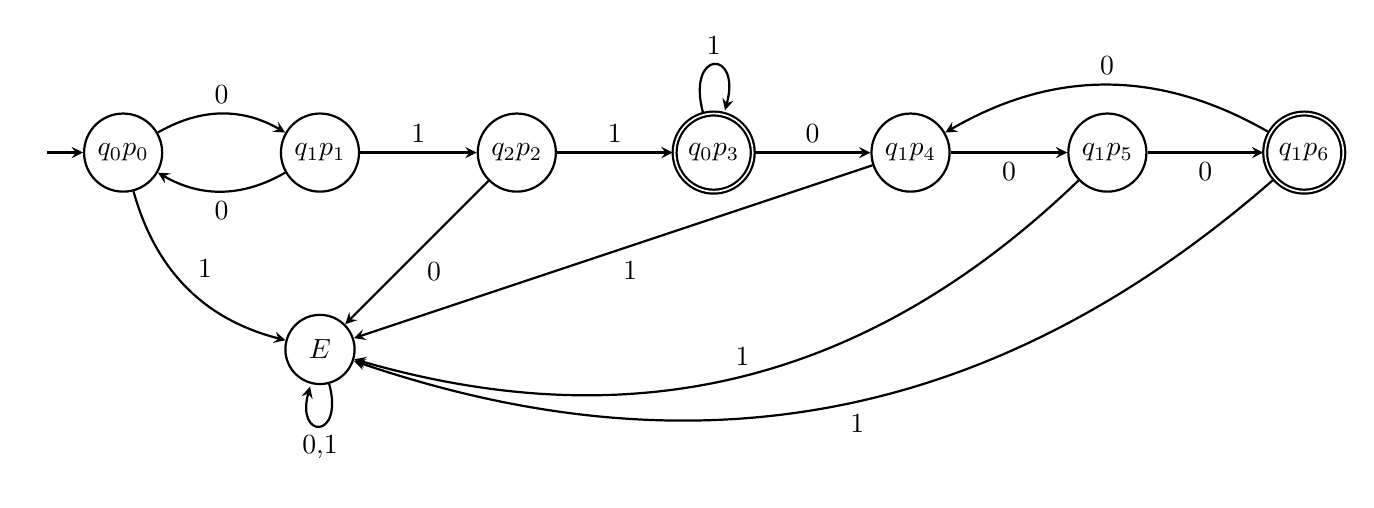
\begin{tikzpicture}[>=stealth,node distance=25mm,on grid,auto, thick, initial text=]
    \node[state,initial] (r00) {$q_0p_0$};
    \node[state] (r11) [right=of r00] {$q_1p_1$};
    \node[state] (r22) [right=of r11] {$q_2p_2$};
    \node[state,accepting] (r03) [right=of r22] {$q_0p_3$};
    \node[state] (r14) [right=of r03] {$q_1p_4$};
    \node[state] (r15) [right=of r14] {$q_1p_5$};
    \node[state,accepting] (r16) [right=of r15] {$q_1p_6$};
    \node[state] (e) [below=of r11] {$E$};
    
    \path[->]
    (r00) edge [bend left] node {0} (r11)
    (r00) edge [bend right] node {1} (e)
    
    (r11) edge [bend left] node {0} (r00)
    (r11) edge node {1} (r22)

    (r22) edge node {0} (e)
    (r22) edge node {1} (r03)

    (r03) edge node {0} (r14)
    (r03) edge [loop above] node {1} (r03)

    (r14) edge node [below] {0} (r15)
    (r14) edge node {1} (e)

    (r15) edge node [below] {0} (r16)
    (r15) edge [bend left] node [above] {1} (e)

    (r16) edge [bend right] node [above] {0} (r14)
    (r16) edge [bend left] node {1} (e)

    (e) edge [loop below] node {0,1} (e);
    
  \end{tikzpicture}

\end{document}